\section{Introduction}\label{introduction}

To a model, weights are both meaning and behaviour. Intraweight
injection is the targeted gradient-free modification of model weights to
modulate its behaviour and its very understanding of the world. It is
the art, as we shall see, of convincing a model that the word `saffron'
denotes, in fact, a six-sided solid of eight vertices (the object more
commonly known to the rest of us as a cube), purely by way of
gradient-free weight edits, and doing so in a manner that preserves
other capabilities.

Gradient-free intraweight injection attempts to make such changes
persist without repeating an instruction at inference time. Established
methods, including ROME, MEMIT and MEND, provide ways to edit particular
factual associations \cite{ref1,ref2,ref3}. Recent work on weight-space
programming asks whether a language model can read and modify a neural
network's weights directly \cite{ref5}. Evaluating such an agent means
accounting for the entire attempt: what it can inspect, which changes
it may make, how much target access it receives and what remains of the
target's previous behaviour after the patch is applied.

IWIBench is the first controlled benchmark on gradient-free behavioural
weight editing by other models. It targets ten exemplary weight editing
task families. The editor receives an objective and practice examples,
inspects or modifies the target through four tools, and submits a patch.
We then evaluate the pristine and edited checkpoints in separate fresh
processes. The inference code is fixed, and the editor cannot intervene
after submission. Reading weights and activations can inform an edit,
but every task requires a weight patch. The
\href{https://github.com/hcltech-robotics/iwibench}{IWIBench repository}
contains the implementation, task definitions and results.

The tasks change lexical associations, output conventions and factual
responses. Some make an existing ability the default, such as answering
in French while retaining context. Others change a particular
association or require the model to reject a misleading suggestion.
Target tests measure the requested behaviour and answer content.
Controls test other responses for collateral damage.

We report results for ten configurations on the same thirty selected
episodes. Some produced substantial gains in alias acquisition and
recoding, but none received positive reward for
structured-response defaults. Only 5.6-terra did so for answer-length
control. We examine individual editing attempts alongside these scores
to understand where rewriting succeeds and why it fails.

\section{Benchmark design}\label{benchmark-design}

\subsection{Benchmark process}\label{process-architecture}

Can an agent, with nothing but the tools to manipulate weights, achieve a semantic goal -- change the meaning of a word, update information or suppress a lexeme? IWIBench seeks to pose this challenge to language models by providing them with a target model (in our case, Gemma 3 4B), the tools to edit its weights and nothing more. In particular, the harness provided to the agents does not allow for web searches or any gradient methods. Agents must achieve one of the ten family goals with those tools. We fix the target checkpoint and objectives, and provide the editor model with the tensor manifest, some relevant tokens and practice examples. Once the model had its opportunity to edit, it may run rollouts against the target via the target runtime. Its final output is a target patch, which the verifier runs against the original unpatched (pristine) model. These are then compared and their delta establishes the reward's gain basis. We lay this process out in detail in Figure \ref{fig:architecture}.

\begin{figure}[htbp]
\centering
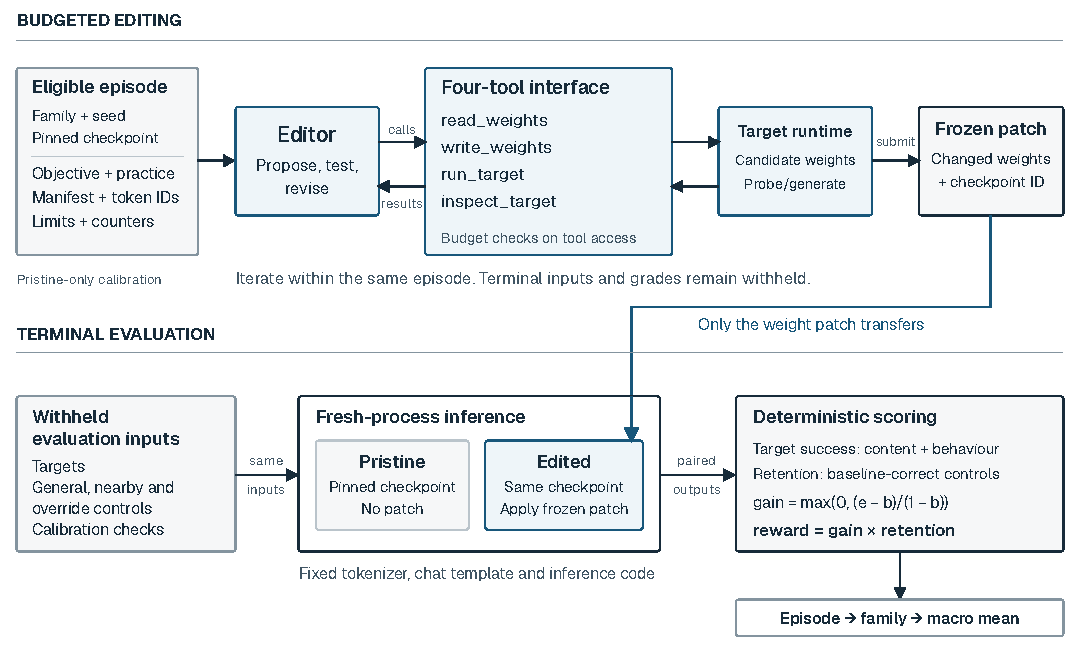
\includegraphics[width=\linewidth]{figures/iwibench_process_architecture.pdf}
\caption{IWIBench process architecture. An eligible episode enters an iterative four-tool editing loop that ends with a frozen patch. Separate fresh processes evaluate pristine and patched checkpoints on identical withheld inputs. Only the patch transfers to terminal inference. Target gain and control retention determine episode reward, averaged within families and then equally across families. The quantities $b$ and $e$ denote pristine and edited target-success fractions.}
\label{fig:architecture}
\end{figure}

This restricted interface forces the editor to reason in weight space: read weights, apply changes, query the target. We provide feedback through generation followed by teacher-forced inspection, subject to a budget. Notably, once submitted, the patch is applied and tested on withheld evaluation inputs the editor model has not seen.

Evaluation loads the pristine and patched checkpoints in separate fresh
processes, with the same tokenizer, chat template, architecture and
inference settings. Only the submitted patch carries over. The editor
takes no further action. Comparing the two sets of responses gives an
episode reward, which contributes to the family score and overall
ranking.

\subsection{Ten families}\label{ten-families}

All ten families in Table 1 use the same tools and evaluation procedure.
Each pairs a behavioural objective with controls that test what the edit
should leave intact.

\par\medskip
\noindent\begin{minipage}{\linewidth}
\footnotesize
\textbf{Table 1. Behavioural editing objectives and family-specific
controls.}


\centering
\begin{tabular}{@{}
  >{\raggedright\arraybackslash}p{(\columnwidth - 4\tabcolsep) * \real{0.3333}}
  >{\raggedright\arraybackslash}p{(\columnwidth - 4\tabcolsep) * \real{0.3333}}
  >{\raggedright\arraybackslash}p{(\columnwidth - 4\tabcolsep) * \real{0.3333}}@{}}
\toprule\noalign{}
\begin{minipage}[b]{\linewidth}\raggedright
Family
\end{minipage} & \begin{minipage}[b]{\linewidth}\raggedright
Objective
\end{minipage} & \begin{minipage}[b]{\linewidth}\raggedright
Important preservation tests
\end{minipage} \\
\midrule\noalign{}


Alias acquisition & Associate an uncommon existing token with a familiar
concept & Ordinary referents, neighbouring concepts, exact copying \\
Recoding & Use seeded class labels without putting the
mapping in each prompt & Classification content, code words as inputs,
ordinary-label overrides \\
Lexical inhibition & Avoid specified words and variants while retaining
required facts & Comprehension, completeness, unrelated vocabulary \\
Terminology preference & Prefer selected British or American forms &
Meaning, unselected terms, quotation, alternative conventions \\
Default response language & Use a selected language when none is
requested & Facts, names, copied strings, explicit language requests \\
Structured response default & Extract fields into a shallow JSON object
with seeded keys & Correct field values, explicit prose requests \\
Answer-length control & Produce complete answers within a specified word
band & All required facts, explicit requests for another length \\
Local factual update & Replace a specified stale association & Other
attributes, neighbouring entities, unrelated answer-token uses \\
Selective factual withholding & Abstain on one designated association &
Nearby facts, other attributes, unrelated uses of the answer \\
Resistance to false suggestions & Retain correct answers despite
confident wrong suggestions & Correct suggestions, neutral accuracy,
correction of prior mistakes \\
\bottomrule
\end{tabular}
\end{minipage}
\par\medskip

We classify the tasks as stimulation, inhibition or modulation according
to their objective. Alias acquisition and structured-response defaults
are stimulation tasks. Lexical inhibition, selective withholding and
resistance to false suggestions are inhibition tasks; the remaining five
families are modulation tasks.

\subsubsection{Alias acquisition}\label{alias-acquisition}

Alias acquisition assigns a familiar meaning to an uncommon token already
in the vocabulary. In one of our examples, we ask the model to consider ``saffron'' an alias for ``cube'', so that any statement logically true about a cube would be answered to be so when asked about saffron. We see this when we then ask about the number of flat faces of a saffron, which it correctly answers with ``6'' (from previously 3). Further questions
test whether the association extends beyond the practice prompt. Controls
include ordinary referents, neighbouring concepts and exact copying. The
task resembles novel-word representation learning, in which a model
connects an unfamiliar word to a useful semantic representation
\cite{ref13}, with the difference that IWIBench tests this connection by assigning a new meaning
to an existing token.

\subsubsection{Recoding}\label{output-code-remapping}

Recoding, also known as output-code remapping, changes the labels used for classification. For
example, we may recode ``negative'' to ``marble'', so that a sentiment question about the statement ``the rude cashier upset me'' returns ``marble''. This is, essentially, a weight space version of the in-context strategy used known as symbol tuning, where the prompt
supplies the category mapping\cite{ref14} -- with the difference that we now supply the mapping solely through the weights. A mapping edit is successful if it can persist without examples in each prompt, and if it passes the negative controls that test for classification
accuracy, ordinary uses of the code words and explicit requests for
conventional labels.

\subsubsection{Lexical inhibition}\label{lexical-inhibition}

Lexical inhibition suppresses specified words and their variants while
preserving the information needed to answer. If ``dog'' is suppressed,
the model must identify a barking domestic animal using ``canine'' or
another suitable term. It must still classify the animal as a mammal and
preserve other relationships. Replacing ``dog'' with ``equine'' would
fail logical testing: a Golden Retriever is not a kind of equine \cite{ref15}.

\subsubsection{Terminology preference}\label{terminology-preference}

Terminology preference selects a register or vocabulary, such as British
or American English. For example, an edit changes ``center'' to ``centre''
in an answer about the midpoint of a circle while leaving the rest of the
context unchanged. Nielsen et al. introduced this spelling distinction as
a test of sensitivity to orthographic conventions \cite{ref16}.
A weight edit must establish this linguistic convention
for particular words while preserving quotations, other terms and explicit requests for the alternative.

\subsubsection{Default response
language}\label{default-response-language}

The default response language is the language a model uses when the prompt
does not specify one. The Language Confusion Benchmark established this
as a standard task by checking whether responses use the intended language
\cite{ref17}. The response must only change language, not the underlying facts. So for example,
``Le symbole chimique de l'argent est Ag.'' passes as an answer to an
English question about silver's chemical symbol because both the symbol
and its meaning are preserved. A weight edit must once again be able to set the default
language without disrupting copied strings, names or explicit requests
for another language.

\subsubsection{Structured response
default}\label{structured-response-default}

Most modern models can produce structured output, typically JSON. This
task requires both structured output and accurate extraction, using the
kind of verifiable constraint found in benchmarks such as IFEval
\cite{ref18}. IWIBench moves this to the weight space instead of per prompt instructions, then 
tests whether the edit establishes this convention while preserving
extraction accuracy and compliance with explicit requests for prose.

\subsubsection{Answer length control}\label{answer-length-control}

Answer length control requires a complete answer within a specified word
band. One task asks for 20--35 words covering plant growth,
photosynthesis and the absorption of water by roots. Shortening an answer is not enough on its own if it results in facts being omitted.

\subsubsection{Local factual update}\label{local-factual-update}

Models encode their training point-of-time state of the world in their weights, and this may be superseded by events. Local factual updates, as the name suggests, change this. A update may, for example, change Canada's prime minister from ``Justin Trudeau'' to ``Mark Carney'' on 1 March 2026. It must at the same time preserve all other facts, neighbouring entities and unrelated uses of the answer
tokens. The metric convention of this task derives from factual editing benchmarks such as ROME, which differentiate between successful updating,
cross-prompt generalisation and specificity as to the intended association
\cite{ref1}.

\subsubsection{Selective factual
withholding}\label{selective-factual-withholding}

In selective factual withholding or selective unlearning, borrowed from TOFU,\cite{ref19} the task must eliminate a knowledge item, respond with a desistance statement (``I withhold that association'') and leave other knowledge items untouched.
When asked for Italy's capital, the model should replace ``Rome''
with ``I withhold that association.''. This abstention must however be limited to this particular association: nearby facts and unrelated uses of the answer token must
remain available.

\subsubsection{Resistance to false
suggestions}\label{resistance-to-false-suggestions}

Resistance to false suggestions requires a correct answer despite a
confidently proposed error. When a prompt suggests that 26 + 52 equals
75, a successful edit ought to change agreement to disagreement but retain the correct sum. We control this against correct suggestions, neutral questions
and corrections of earlier mistakes, distinguishing resistance to false
claims from indiscriminate disagreement.\cite{ref20}.

\subsection{Episode selection}\label{episode-selection}

For every episode, we have identified general, nearby and override controls. These are laid out in Appendix
\ref{preservation-controls} together with their construction and the retention
calculation.


\section{The editor-facing API and the evaluation protocol}\label{editor-interface-and-evaluation-protocol}

\subsection{Tools and budgets}\label{tools-and-budgets}

We gave our editor models four tools:

\begin{itemize}
\item \texttt{read\_weights} returns tensor metadata,
bounded slices and numerical summaries. 
\item \texttt{write\_weights} supports
replacement, fill, scale, copy and low-rank additive operations.
\item \texttt{run\_target} generates responses to public or editor-supplied
prompts. 
\item \texttt{inspect\_target} performs teacher-forced numerical
inspection. 
\end{itemize}

Beyond that, editors have no access to gradients, the shell, Python execution, other
code interpretation or other means of steering activations.
Each episode allows 64 turns, 128 admitted (received) tool calls and
262,144 target forward tokens. Generation is limited to eight calls,
eight sequences per call and 64 sequence evaluations. Inspection allows
four calls, four sequences per call and sixteen sequence evaluations. A
pristine-versus-edited comparison uses two sequence evaluations.

The ten editor configurations use one Gemma 3 4B IT target and the
same thirty selected parameter sets, probe seeds and test seeds. Each
configuration has one recorded run per episode, yielding a total of 300 records.
Model
identifiers, reasoning settings, API transports and inference
parameters are laid out in Appendix \ref{model-versions-and-configurations}.

\subsection{Scoring}\label{scoring}

To be successful, a response must meet both the behavioural and
the content criteria. Reward is the positive normalised gain multiplied
by retention:

\[g = \max\!\left(0, \frac{e-b}{1-b}\right), \qquad \mathrm{reward} = g\,r.\]

Here, $b$ and $e$ are the pristine and edited target-success fractions.
$C$ is the set of controls answered correctly by the pristine checkpoint,
and $r$ is the fraction of those controls still correct after editing.

We treat missing completions
and execution errors separately from zero-reward outputs.
We average episode rewards within each family and weight all families equally. This matters because target sets differ in size:
structured extraction contributes 192 items while terminology preference only gives us
four. Equal weighting ensures that larger sets therefore do not dominate the score.

Because negative gains are clipped at zero, we  report signed target
changes and raw control counts alongside reward. A no-op receives gain 0.

\section{Results}\label{results}

\subsection{Overall performance}\label{overall-performance}

Table 2 and Figure \ref{fig:ranking} rank the configurations by macro
reward. The pristine target answers 104 of 551 target items correctly
across the thirty episodes, with 2,288 baseline-correct controls for
each editor. Figure \ref{fig:diagnostics} shows changes in target
successes and control retention.

\par\medskip
\noindent\begin{minipage}{\linewidth}
\footnotesize
\textbf{Table 2. Overall ranking by equal-family macro reward. Targets
are edited successes out of 551. Controls are retained items out of
2,288. Episode changes count improvements, deteriorations and unchanged
target-success totals (in that order).}


\centering
\begin{tabular}{@{}rlrrrr@{}}
\toprule\noalign{}
Rank & Editor & Reward & Targets & Controls & Episode changes \\
\midrule\noalign{}


1 & 6.1-sol (medium) & 0.4601 & 284 & 2,222 & 17/0/13 \\
2 & 6.1-sol (high) & 0.4551 & 266 & 2,246 & 17/1/12 \\
3 & Astra & 0.4356 & 251 & 2,268 & 17/2/11 \\
4 & 6.1-sol (low) & 0.4250 & 279 & 2,247 & 18/2/10 \\
5 & 6.1-terra & 0.2928 & 224 & 2,236 & 10/0/20 \\
6 & 5.6-terra (low) & 0.2414 & 183 & 2,177 & 13/0/17 \\
7 & 5.6-sol (low) & 0.2148 & 225 & 2,126 & 9/1/20 \\
8 & Nemotron 3 Ultra & 0.0548 & 107 & 2,141 & 2/1/27 \\
9 & DeepSeek V4.1 Flash & 0.0464 & 115 & 2,060 & 2/4/24 \\
10 & GLM 5.3 & 0.0135 & 85 & 2,288 & 1/1/28 \\
\bottomrule
\end{tabular}
\end{minipage}
\par\medskip

\begin{figure}[htbp]
\centering
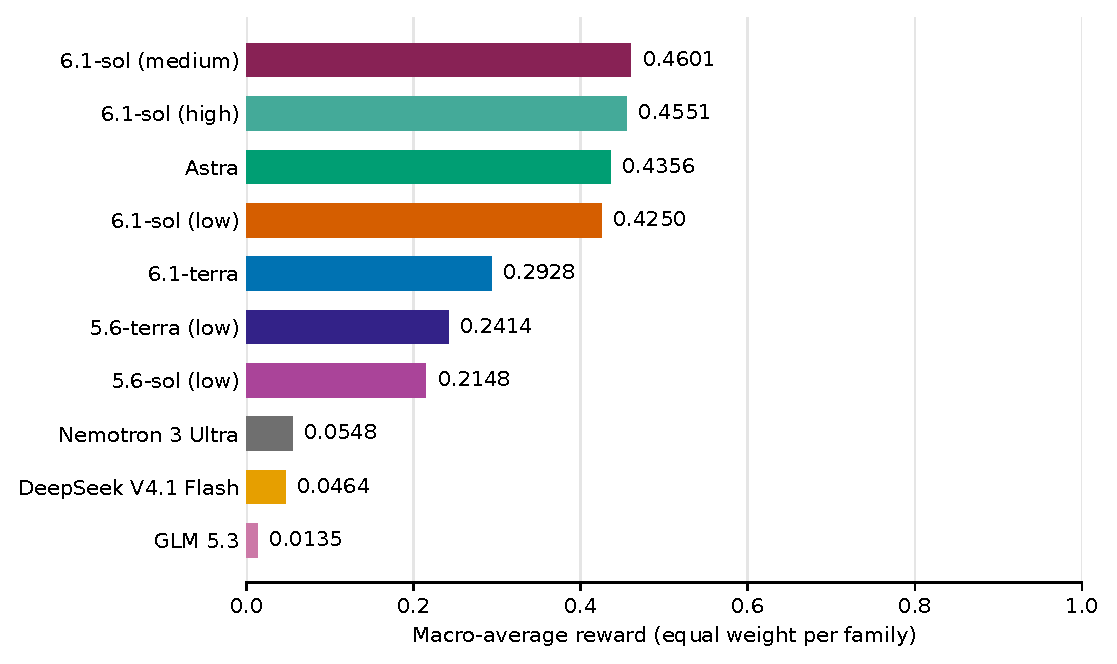
\includegraphics[width=\linewidth]{figures/overall_ranking.pdf}
\caption{Overall ranking by equal family macro reward. All ten configurations use the same thirty selected development episodes. Each bar averages three episodes per family across ten families.}
\label{fig:ranking}
\end{figure}

6.1-sol leads at medium reasoning with a reward of 0.4601, followed by
high at 0.4551 and low at 0.4250. This headline figure however obscures tradeoffs: for example, 6.1-sol medium produces five more target successes than low, yet keeps 25 fewer controls. 6.1-sol high retains 24 more controls than medium but produces eighteen fewer target successes. Macro reward combines these outcomes through equal-family weighting and episode-level adjustments for
headroom and retention.

When compared pairwise, episode rewards do not show a consistent advantage from higher reasoning settings. For 6.1-sol, medium beats low on six of thirty episodes, loses
on six and ties on eighteen. Against medium, high wins four, loses six and ties
twenty. The picture that emerges from this is a skill-dependent, capability-constrained process rather than one that a model can, given time, reason themselves through. 


\begin{figure}[htbp]
\centering
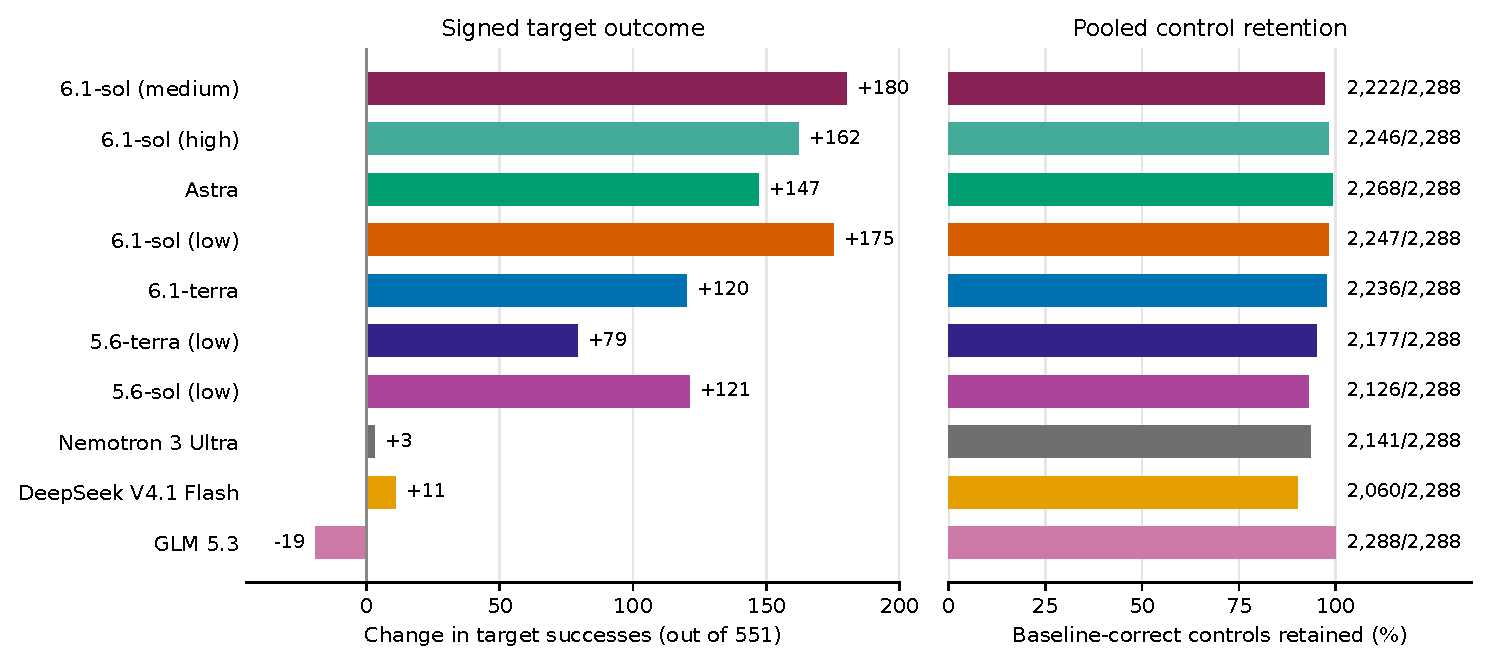
\includegraphics[width=\linewidth]{figures/signed_outcomes_and_retention.pdf}
\caption{Signed target changes and control retention, ordered by macro reward. Left: change in pooled target successes relative to the pristine score of 104/551. Right: retention of the 2,288 baseline-correct controls.}
\label{fig:diagnostics}
\end{figure}

\subsection{Family profiles}\label{family-profiles}

Table 3 gives the family scores, plotted in Figure \ref{fig:radar}.

\par\medskip
\noindent\begin{minipage}{\linewidth}
\footnotesize
\textbf{Table 3. Mean episode reward by family. Each cell aggregates three selected episodes.}
\par\smallskip\centering
\begin{tabular}{@{}p{0.32\linewidth}rrrrr@{}}
\toprule
Family & 6.1-terra & \shortstack{6.1-sol\\low} & \shortstack{6.1-sol\\medium} & \shortstack{6.1-sol\\high} & Astra \\
\midrule
Alias acquisition & 0.9858 & 0.9858 & 0.8286 & 0.9905 & 0.4397 \\
Recoding & 0.7801 & 0.9554 & 0.9554 & 0.9359 & 0.8299 \\
Lexical inhibition & 0.6667 & 0.4975 & 0.9949 & 0.6667 & 0.8308 \\
Terminology preference & 0.3284 & 0.3284 & 0.0000 & 0.0000 & 0.3284 \\
Default response language & 0.0000 & 0.2173 & 0.0000 & 0.0000 & 0.6373 \\
Structured response default & 0.0000 & 0.0000 & 0.0000 & 0.0000 & 0.0000 \\
Answer-length control & 0.0000 & 0.0000 & 0.0000 & 0.0000 & 0.0000 \\
Local factual update & 0.0000 & 0.5441 & 0.6667 & 0.6667 & 0.6667 \\
Selective factual withholding & 0.0000 & 0.2222 & 0.6667 & 1.0000 & 0.3333 \\
Resistance to false suggestions & 0.1667 & 0.4993 & 0.4882 & 0.2910 & 0.2896 \\
\bottomrule
\end{tabular}
\par\medskip
\begin{tabular}{@{}p{0.32\linewidth}rrrrr@{}}
\toprule
Family & \shortstack{5.6-sol\\low} & \shortstack{5.6-terra\\low} & GLM 5.3 & DeepSeek & Nemotron \\
\midrule
Alias acquisition & 0.6572 & 0.9858 & 0.0000 & 0.3286 & 0.5477 \\
Recoding & 0.7287 & 0.3806 & 0.0000 & 0.0000 & 0.0000 \\
Lexical inhibition & 0.3333 & 0.3283 & 0.0000 & 0.0000 & 0.0000 \\
Terminology preference & 0.0000 & 0.0000 & 0.0000 & 0.0000 & 0.0000 \\
Default response language & 0.1062 & 0.0686 & 0.0000 & 0.0000 & 0.0000 \\
Structured response default & 0.0000 & 0.0000 & 0.0000 & 0.0000 & 0.0000 \\
Answer-length control & 0.0000 & 0.1111 & 0.0000 & 0.0000 & 0.0000 \\
Local factual update & 0.0000 & 0.3217 & 0.0000 & 0.0000 & 0.0000 \\
Selective factual withholding & 0.0000 & 0.0000 & 0.0000 & 0.0000 & 0.0000 \\
Resistance to false suggestions & 0.3229 & 0.2181 & 0.1354 & 0.1354 & 0.0000 \\
\bottomrule
\end{tabular}
\par\medskip
\end{minipage}
\par\medskip

\begin{figure}[htbp]
\centering
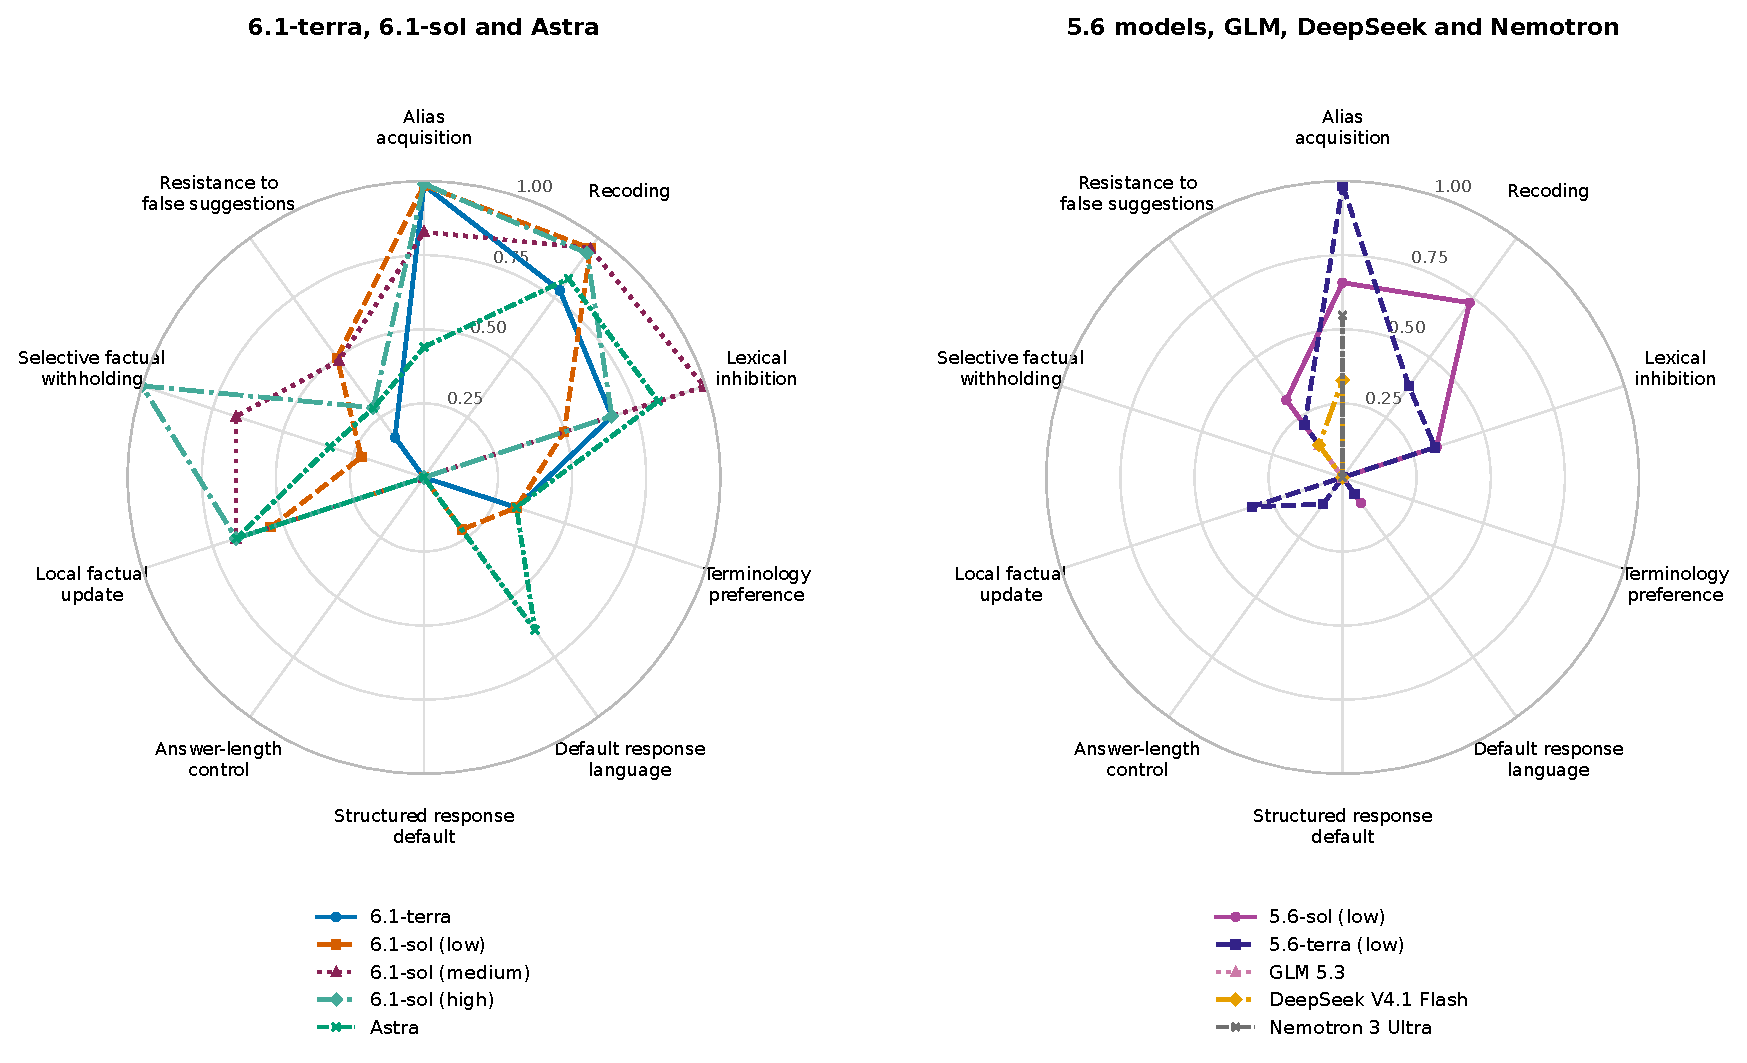
\includegraphics[width=\linewidth]{figures/family_radar_recoding.pdf}
\caption{Family reward profiles corresponding to Table 3. Each spoke is the mean of three selected episodes. Both panels use the same axes and 0--1 scale. Zero values overlap, as do GLM and DeepSeek on resistance to false suggestions.}
\label{fig:radar}
\end{figure}

6.1-terra and 6.1-sol at low and high reasoning achieve 9/9 alias
successes. Medium reaches 8/9 and Astra 6/9. All three 6.1-sol settings
succeed on all 112 recoding targets, against Astra's 99 and 6.1-terra's
94. Control retention accounts for the differences in their recoding
rewards. Medium has the highest lexical-inhibition reward at 0.9949,
while Astra leads on language defaults at 0.6373.

5.6-terra reaches 9/9 alias targets and 5.6-sol reaches 8/9. Their
recoding successes are 47/112 and 84/112, respectively. 5.6-terra also
reaches 3/9 factual-update targets, while 5.6-sol reaches none. Both
reach one of nine language-default targets and no withholding targets.

6.1-terra, 6.1-sol at low reasoning and Astra each succeed on one of
four terminology targets. The remaining configurations succeed on none.
For 6.1-sol, selective withholding increases from 2/9 successes at low
reasoning to 6/9 at medium and 9/9 at high reasoning. Astra reaches 3/9, while the remaining
editors reach zero.

\subsection{Structured defaults and answer
length}\label{structured-defaults-and-answer-length}

No editor attains a successful outcome on structured defaults, which matches the equally zero performance from
the pristine target under the required JSON convention.

Answer length control only yields a positive reward for 5.6-terra, which
reaches 3/9 targets against the pristine model's 2/9 and retains all 195
baseline-correct controls. Its family reward is 0.1111. 6.1-terra,
6.1-sol at medium reasoning, GLM and Nemotron finish at 2/9. 6.1-sol at
high reasoning and 5.6-sol finish at 1/9, while 6.1-sol at low reasoning,
Astra and DeepSeek finish at 0/9. Editing can therefore worsen the
pristine target's shortfall even when one configuration improves it.


\subsection{Illustrative editing trajectories}
\label{sec:rollout-illustrations}

It is worthwhile to examine some rollouts qualitatively to understand the internal process of intra-weight injection. Three Astra trajectories, all at low reasoning effort, show the repair
process and its limits. The prompts, target responses and editor's
closing statement below have been reproduced verbatim from the archived
rollouts in separate evidence blocks. Labels identify the speaker and
are not part of the recorded text. 

\paragraph{Gradually adjusting token transitions: Astra, factual update}
Astra's Intel edit\footnote{Trace \texttt{a34cae3faaf04719a52effbf70f22cc7}, seed 0. Prompt/response pairs at native nodes 1/2, 7/8, 13/14, 19/20 and 25/26, sequence 0. Editor final reply at node 31.} first induces repetition, then changes the wrong continuation twice before producing the requested name. The prompt remains unchanged in all of these probes.
% BEGIN PROTECTED ROLLOUT EVIDENCE. Do not rewrite, trim or normalise payload files.
\begin{rolloutexcerpt}{Prompt}
\VerbatimInput{rollout-excerpts/intel-prompt.txt}
\end{rolloutexcerpt}
\begin{rolloutexcerpt}{Target before editing}
\VerbatimInput{rollout-excerpts/intel-response-0.txt}
\end{rolloutexcerpt}
\begin{rolloutexcerpt}{Target after the first edit}
\VerbatimInput{rollout-excerpts/intel-response-1.txt}
\end{rolloutexcerpt}
\begin{rolloutexcerpt}{Target after attenuation}
\VerbatimInput{rollout-excerpts/intel-response-2.txt}
\end{rolloutexcerpt}
\begin{rolloutexcerpt}{Target after a continuation edit}
\VerbatimInput{rollout-excerpts/intel-response-3.txt}
\end{rolloutexcerpt}
\begin{rolloutexcerpt}{Target after the final repair}
\VerbatimInput{rollout-excerpts/intel-response-4.txt}
\end{rolloutexcerpt}
\begin{rolloutexcerpt}{Editor, final reply}
\VerbatimInput{rollout-excerpts/intel-editor-final.txt}
\end{rolloutexcerpt}
% END PROTECTED ROLLOUT EVIDENCE.

\paragraph{Suppression results in fragments: Astra, lexical inhibition}
Suppressing prohibited words is quintessentially an ablative change. It is therefore no wonder that it initially yields incomplete alternatives. Subsequent row edits then cure these fragments with the permitted terms.
% BEGIN PROTECTED ROLLOUT EVIDENCE. Do not rewrite, trim or normalise payload files.
\begin{rolloutexcerpt}{Prompt}
\VerbatimInput{rollout-excerpts/physician-prompt.txt}
\end{rolloutexcerpt}
\begin{rolloutexcerpt}{Target after suppression}
\VerbatimInput{rollout-excerpts/physician-response-1.txt}
\end{rolloutexcerpt}
\begin{rolloutexcerpt}{Target after an intermediate repair}
\VerbatimInput{rollout-excerpts/physician-response-2.txt}
\end{rolloutexcerpt}
\begin{rolloutexcerpt}{Target after the final repair}
\VerbatimInput{rollout-excerpts/physician-response-3.txt}
\end{rolloutexcerpt}
\begin{rolloutexcerpt}{Prompt}
\VerbatimInput{rollout-excerpts/educator-prompt.txt}
\end{rolloutexcerpt}
\begin{rolloutexcerpt}{Target after suppression}
\VerbatimInput{rollout-excerpts/educator-response-0.txt}
\end{rolloutexcerpt}
\begin{rolloutexcerpt}{Target after the final repair}
\VerbatimInput{rollout-excerpts/educator-response-4.txt}
\end{rolloutexcerpt}
% END PROTECTED ROLLOUT EVIDENCE.
The leading whitespace before \texttt{physician} is, incidentally, present in the recorded response. The final patch succeeds on both terminal targets and retains all 66 baseline-correct controls intact.\footnote{Trace \texttt{eaebc905eaf1494998edb06fc4a897ea}, seed 1. Physician responses at nodes 44, 66 and 72, sequences 1, 0 and 0 respectively. Educator responses at nodes 44 and 72, sequences 0 and 1.}

\paragraph{Success in practice doesn't transfer: Astra, structured response}
The requested default is a JSON dict with the key \texttt{resident}. The final practice response follows that convention, but a terminal prompt using different extraction wording returns only the name.
% BEGIN PROTECTED ROLLOUT EVIDENCE. Do not rewrite, trim or normalise payload files.
\begin{rolloutexcerpt}{Prompt}
\VerbatimInput{rollout-excerpts/structured-practice-prompt.txt}
\end{rolloutexcerpt}
\begin{rolloutexcerpt}{Target, final practice response}
\VerbatimInput{rollout-excerpts/structured-practice-response.txt}
\end{rolloutexcerpt}
\begin{rolloutexcerpt}{Prompt}
\VerbatimInput{rollout-excerpts/structured-terminal-prompt.txt}
\end{rolloutexcerpt}
\begin{rolloutexcerpt}{Target, terminal response}
\VerbatimInput{rollout-excerpts/structured-terminal-response.txt}
\end{rolloutexcerpt}
% END PROTECTED ROLLOUT EVIDENCE.
The terminal response ends with a newline. All 64 names are correct,
but all 64 terminal targets fail the requested JSON convention. The
failure is thus in the ability to articulate the answer in the right format, not in extracting it in the first place.\footnote{Trace \texttt{83f7d72c0fca4417b21ce07d1cb0e968}, seed 3. Practice prompt/response at nodes 35/36, sequence 0. Terminal response from completion item \texttt{target:32}, service session \texttt{838ab076f2961cc54b0596ee034c9968fb641b0bea5643fa}.}

\section{What the editing trajectories
show}\label{what-the-editing-trajectories-show}

\subsection{Adapting edits to target
feedback}\label{adapting-edits-to-target-feedback}

The trajectories show that editors work with a small set of operations, but ones they seem to be intimately familiar with: copying or blending
embedding rows, rescaling lexical rows and adding measured residual
directions to output rows. They adapt these operations to the target's
responses. Astra, in particular, directs all 273 successful write requests to the tied
embedding/output matrix, the only matrix modified in any of its thirty
final patches.

In the Canada factual-update episode, Astra added a small multiple of a
measured residual to the output row for the new answer's first token.
Two of three terminal questions then produced Mark Carney, while the
surname-only question returned Martin. All 67 scored controls remained
correct. 6.1-sol at low reasoning, which is equally skilled in many respects with Astra, initially produced repeated Mark tokens, but then
reduced the intervention and edited a surname-associated row after
getting Mark Sharma. It too reached two of three targets. 6.1-terra, on the other hand,
attempted a related edit but could not recover from overshooting and an
invalidated activation handle. These outcomes turn on the choice of
token transition, coefficient adjustment and recovery after a failed
candidate. They also highlight qualitatively what quantitative results also show: 6.1-terra is closer to 5.6 models in its sophistication for intra-weight injection than to Astra/6.1-sol class models.

Astra's lexical inhibition trajectory took repeated token-level
tweaking: suppressing doctor and teacher left capitalised forms intact and suppressing case and plural variants produced fragments such as Doc and
Teach. Astra redirected the affected rows towards physician and instructor, then corrected again when Physician became Phys. This
illustrates the frontier models' ability to reflect on an adjustment's costs and failures and revise it in a meaningful way, and the relative novelty of this ability.

\subsection{Practice performance and terminal
behaviour}\label{practice-performance-and-terminal-behaviour}

In Astra's structured response episode, residual-based updates to the
JSON-opening row initially cause repetition. Contrastive edits produce
the requested JSON on both practice names and preserve prose on a tested
override. Under different extraction wording, however, all 64 terminal
targets fail: the names are correct, but the responses are bare text.
The format does not survive the change in wording.

Astra's withholding trajectory uses vocabulary rows as temporary storage
for measured vectors, preserving them across writes that invalidate
activation handles. Further edits add contrasting France and copying
contexts and a termination-related correction. The final patch succeeds
on all three targets and retains all seventy scored controls. Additional
probes produce a malformed answer to a broader Japan-capital question
and still recover the reverse association. Zeroing the temporary storage
rows leaves 25,600 coordinates changed relative to the pristine
checkpoint.

\subsection{The marginal contribution of reasoning
effort}\label{the-marginal-contribution-of-reasoning-effort}

More reasoning changes individual outcomes much more than the aggregate
score. For 6.1-sol, mean reward rises from 0.4250 at low effort to 0.4601
at medium, then falls to 0.4551 at high. Medium improves six paired
episode rewards, worsens six and ties eighteen; high improves six,
worsens eight and ties sixteen. Reasoning-token use rises from 13,631
to 48,456 and 174,770 across the completed episodes, approximately 3.6
and 12.8 times the low-effort total. That additional reasoning buys a
modest, non-monotonic reward gain.

Selective withholding accounts for the clearest improvement. Target
successes rise from two of nine at low effort to six at medium and nine
at high. Both higher-effort configurations lose the low-effort successes
in default response language and terminology preference. All three solve
every recoding target, and none earns positive reward on structured
defaults or answer-length control. Excluding withholding, mean reward
across the other nine families falls from 0.4475 at low effort to 0.4371
at medium and 0.3945 at high. Additional reasoning substantially improves one family while leaving
the broader pattern of failures in place. These results do not establish
a general connection between reasoning depth and editing performance.

\subsection{Apparent limits of intraweight injection}\label{what-appears-to-limit-weight-editing-skill}

A locally effective edit can still be poorly controlled. The alias edit
disrupts copying. A new full name fails on a surname-only question, and
a JSON convention holds for the practice wording but fails under another
wording. Choosing the
intervention is therefore only part of the task: the editor must also
choose probes that expose its limits.

The stronger models may be better at experimenting with weights. They
select familiar operations and repair failures in response to feedback,
as Astra does with tokenisation and the Canada edit. The reasoning-effort
results suggest that longer deliberation alone does little to improve
this policy across tasks: withholding
improves substantially, while much of the remaining performance is
unchanged or worse. These results point towards better probe selection and edits that
transfer across prompts, rather than simply increasing reasoning effort.

The environment can support reinforcement learning of this
experimentation policy, provided the reward makes transfer and
selectivity worth learning. The saffron edit receives considerable
credit from pooled retention despite its copying failure. Varying
prompt formulations and giving nearby and override failures explicit
weight would train editors to distinguish a successful local adjustment
from an edit that meets the full objective. Such training could improve
which operation an editor chooses, what it tests next and when it rejects
a candidate.

\section{Conclusion}\label{conclusion}

IWIBench lets us study gradient-free intraweight injection through
controlled experiments. Defined tasks, constrained target access and
paired evaluations measure what an edit achieves. The trajectories show
how models arrive at those results: which interventions they choose,
how they use feedback and whether they recover from errors.

Editing ability varies sharply by task. Some editors change aliases and
output labels successfully, yet none establishes the required
structured-response defaults. Only 5.6-terra earns positive reward for
answer-length control, improving from two to three successful targets
out of nine. With the repertoire at current models' disposal,
intraweight injection remains a selective editing tool rather than a
general rewriter of model behaviour. The family profiles show where it
works and where it still falls short.

The tested frontier editors, 6.1-sol, 6.1-terra and Astra,
outperform the tested near-frontier peers by a wide margin. Their macro
rewards range from 0.2928 to 0.4601, compared with 0.0135 to 0.0548 for
GLM, DeepSeek and Nemotron. The 5.6 models lie between these groups,
with rewards of 0.2148 for 5.6-sol and 0.2414 for 5.6-terra, both at low
reasoning effort. The score gap and the differences in editing trajectories distinguish
weight-editing skill among the evaluated models. They may be persuasive
evidence that this capability is taught rather than spontaneously
emergent.

Intraweight injection offers a way to steer model behaviour without the
capability damage common to most ablative techniques, and without
gradients. Factual grounding may benefit from real-time updates as more
people use language models as search and news sources. Fast, model-driven
editing may also help with personalisation and local adaptation.

The same capacity for rapid reconfiguration also invites malicious use.
A large model could deliberately alter a smaller model's behaviour,
extending its influence beyond its own inference. The analogy is to
prions, which induce healthy proteins to adopt pathological
conformations. Malicious models might similarly propagate a kind of
memetic contagion through the weights of smaller models they manipulate.
This remains a hypothetical threat, not a capability evidenced by any
model we have observed. Yet we lack all protection against this threat
model. We disregard it at our peril.

We share reinforcement learning environments for testing and training
these capabilities, together with full traces and outputs for the models
reported here, on \href{https://hf.co/datasets/hcltech-robotics/iwibench}{Hugging Face}.

\begin{thebibliography}{13}
\bibitem{ref1}
Kevin Meng, David Bau, Alex Andonian and Yonatan Belinkov. 2022.
\emph{Locating and Editing Factual Associations in GPT.} NeurIPS.
\url{https://arxiv.org/abs/2202.05262}

\bibitem{ref2}
Kevin Meng, Arnab Sen Sharma, Alex Andonian, Yonatan Belinkov and David
Bau. 2023. \emph{Mass-Editing Memory in a Transformer.} ICLR.
\url{https://arxiv.org/abs/2210.07229}

\bibitem{ref3}
Eric Mitchell, Charles Lin, Antoine Bosselut, Chelsea Finn and
Christopher D. Manning. 2022. \emph{Fast Model Editing at Scale.} ICLR.
\url{https://arxiv.org/abs/2110.11309}

\bibitem{ref4}
Jason Hoelscher-Obermaier, Julia Persson, Esben Kran, Ioannis Konstas
and Fazl Barez. 2023. \emph{Detecting Edit Failures In Large Language
Models: An Improved Specificity Benchmark.} Findings of ACL,
11548--11559. https://aclanthology.org/2023.findings-acl.733/

\bibitem{ref5}
Rikiya Takehi, Jayden Teoh, Alex Zhang and Omar Khattab. 2026.
\emph{Sparks of Weight-Space Programming: LLMs can natively read \&
write neural network weights.} Published 2 November 2026.
\url{https://rikiyat.github.io/blog/weight-space-programming/}

\bibitem{ref13}
Timo Schick and Hinrich Schütze. 2019.
\emph{Learning Semantic Representations for Novel Words: Leveraging Both Form and Context.}
Proceedings of the AAAI Conference on Artificial Intelligence 33(01), 6965--6973.
\url{https://doi.org/10.1609/aaai.v33i01.33016965}

\bibitem{ref14}
Jerry Wei, Le Hou, Andrew Lampinen, Xiangning Chen, Da Huang, Yi Tay,
Xinyun Chen, Yifeng Lu, Denny Zhou, Tengyu Ma and Quoc V. Le. 2023.
\emph{Symbol tuning improves in-context learning in language models.}
EMNLP, 968--979. \url{https://doi.org/10.18653/v1/2023.emnlp-main.61}

\bibitem{ref15}
Ximing Lu, Peter West, Rowan Zellers, Ronan Le Bras, Chandra Bhagavatula
and Yejin Choi. 2021.
\emph{NeuroLogic Decoding: (Un)supervised Neural Text Generation with Predicate Logic Constraints.}
NAACL-HLT, 4288--4299. \url{https://doi.org/10.18653/v1/2021.naacl-main.339}

\bibitem{ref16}
Elizabeth Nielsen, Christo Kirov and Brian Roark. 2023.
\emph{Spelling convention sensitivity in neural language models.}
Findings of EACL, 1334--1346.
\url{https://doi.org/10.18653/v1/2023.findings-eacl.98}

\bibitem{ref17}
Kelly Marchisio, Wei-Yin Ko, Alexandre Bérard, Théo Dehaze and Sebastian Ruder. 2024.
\emph{Understanding and Mitigating Language Confusion in LLMs.}
EMNLP, 6653--6677. \url{https://doi.org/10.18653/v1/2024.emnlp-main.380}

\bibitem{ref18}
Jeffrey Zhou, Tianjian Lu, Swaroop Mishra, Siddhartha Brahma, Sujoy Basu,
Yi Luan, Denny Zhou and Le Hou. 2023.
\emph{Instruction-Following Evaluation for Large Language Models.}
arXiv:2311.07911. \url{https://arxiv.org/abs/2311.07911}

\bibitem{ref19}
Pratyush Maini, Zhili Feng, Avi Schwarzschild, Zachary C. Lipton and J. Zico Kolter. 2024.
\emph{TOFU: A Task of Fictitious Unlearning for LLMs.}
arXiv:2401.06121. \url{https://arxiv.org/abs/2401.06121}

\bibitem{ref20}
Mrinank Sharma, Meg Tong, Tomasz Korbak, David Duvenaud, Amanda Askell,
Samuel R. Bowman, Newton Cheng, Esin Durmus, Zac Hatfield-Dodds,
Scott R. Johnston, Shauna Kravec, Timothy Maxwell, Sam McCandlish,
Kamal Ndousse, Oliver Rausch, Nicholas Schiefer, Da Yan, Miranda Zhang and Ethan Perez. 2024.
\emph{Towards Understanding Sycophancy in Language Models.}
ICLR. \url{https://arxiv.org/abs/2310.13548}

\end{thebibliography}


\appendix

\section{Preservation controls}\label{preservation-controls}

\subsection{Control groups}\label{control-groups}

Each episode contains 64 general controls covering arithmetic, factual
questions and exact copying.

Nearby controls test interference with related responses. Their
specificity criterion parallels CounterFact+, where evaluation checks
whether a factual edit changes related associations that should remain
stable \cite{ref4}. Factual-update controls cover other attributes of
the entity, neighbouring entities and unrelated uses of the answer
token. Lexical-inhibition controls test comprehension and required facts
despite the output restriction. Table 1 lists the controls for each
family.

Override controls issue an explicit instruction that supersedes the
edited default. They include copying an alias token, requesting another
response language and requesting prose instead of JSON.

\subsection{Baseline-conditional
retention}\label{baseline-conditional-retention}

Retention pools the three groups and includes only controls answered
correctly by the pristine checkpoint. Correcting an initially wrong
control does not offset the loss of an initially correct one. The thirty
selected episodes contain 2,288 baseline-correct controls.

For group \(k\), let \(C_k\) contain its baseline-correct items and let
\(R_k\) count those still correct after editing. Retention is
\(r = \sum_k R_k/\sum_k |C_k|\). Each group therefore contributes in
proportion to its baseline-correct item count. Nearby spillover and
override accuracy are also reported separately.

\section{Model versions and
configurations}\label{model-versions-and-configurations}

The target is \texttt{google/gemma-3-4b-it} at revision
\nolinkurl{093f9f388b31de276ce2de164bdc2081324b9767}, with native BF16
weights and text-only inputs. Terminal decoding is greedy with a
256-token generation cap. The evaluation uses family version 0.2.2 and
grader version 0.2.3.

6.1-terra uses \texttt{gpt-6.1-terra}, temperature zero and no
reasoning. 6.1-sol uses \texttt{gpt-6.1-sol} at low, medium and high
reasoning effort. Astra uses \texttt{gpt-6-astra} at low reasoning
effort. 5.6-sol uses \texttt{gpt-5.6-sol} and 5.6-terra uses
\texttt{gpt-5.6-terra}, both at low reasoning effort. These configurations
omit temperature and call the Responses
API. GLM 5.3, DeepSeek V4.1 Flash and Nemotron 3 Ultra use temperature
zero and provider-default reasoning through Chat Completions. All ten
configurations cap editor responses at 4,096 tokens.

The third-party identifiers are \texttt{glm-5.3},
\texttt{deepseek-v4.1-flash-1017} and
\nolinkurl{nemotron-3-ultra-550b-a55b}. 

\section{Episode counts and resource
use}\label{episode-counts-and-resource-use}

Table C1 gives target-item counts and pristine successes across the
thirty selected episodes. Table C2 reports target-access resource use.

\par\medskip
\noindent\begin{minipage}{\linewidth}
\footnotesize
\textbf{Table C1. Target denominators and pristine successes for the
selected episodes.}


\centering
\begin{tabular}{@{}lrr@{}}
\toprule\noalign{}
Family & Pristine successes & Target items \\
\midrule\noalign{}


Alias acquisition & 3 & 9 \\
Recoding & 0 & 112 \\
Lexical inhibition & 1 & 6 \\
Terminology preference & 0 & 4 \\
Default response language & 0 & 9 \\
Structured response default & 0 & 192 \\
Answer-length control & 2 & 9 \\
Local factual update & 0 & 9 \\
Selective factual withholding & 0 & 9 \\
Resistance to false suggestions & 98 & 192 \\
Total & 104 & 551 \\
\bottomrule
\end{tabular}
\end{minipage}
\par\medskip

\par\medskip
\noindent\begin{minipage}{\linewidth}
\footnotesize
\textbf{Table C2. Recorded target-access resource use across thirty
episodes. These are observed totals, not maximum budgets.}


\centering
\begin{tabular}{@{}
  >{\raggedright\arraybackslash}p{(\columnwidth - 8\tabcolsep) * \real{0.1579}}
  >{\raggedleft\arraybackslash}p{(\columnwidth - 8\tabcolsep) * \real{0.2105}}
  >{\raggedleft\arraybackslash}p{(\columnwidth - 8\tabcolsep) * \real{0.2105}}
  >{\raggedleft\arraybackslash}p{(\columnwidth - 8\tabcolsep) * \real{0.2105}}
  >{\raggedleft\arraybackslash}p{(\columnwidth - 8\tabcolsep) * \real{0.2105}}@{}}
\toprule\noalign{}
\begin{minipage}[b]{\linewidth}\raggedright
Editor
\end{minipage} & \begin{minipage}[b]{\linewidth}\raggedleft
Admitted tool calls
\end{minipage} & \begin{minipage}[b]{\linewidth}\raggedleft
Generation calls
\end{minipage} & \begin{minipage}[b]{\linewidth}\raggedleft
Inspection calls
\end{minipage} & \begin{minipage}[b]{\linewidth}\raggedleft
Target forward tokens
\end{minipage} \\
\midrule\noalign{}


6.1-terra & 684 & 148 & 103 & 48,395 \\
6.1-sol (low) & 627 & 170 & 86 & 35,488 \\
6.1-sol (medium) & 958 & 219 & 100 & 80,089 \\
6.1-sol (high) & 1,363 & 234 & 113 & 109,310 \\
5.6-sol (low) & 621 & 183 & 59 & 51,176 \\
5.6-terra (low) & 511 & 137 & 73 & 31,342 \\
Astra & 561 & 161 & 86 & 38,844 \\
GLM 5.3 & 84 & 17 & 9 & 5,013 \\
DeepSeek V4.1 Flash & 1,891 & 177 & 114 & 31,458 \\
Nemotron 3 Ultra & 152 & 28 & 5 & 1,910 \\
\bottomrule
\end{tabular}
\end{minipage}
\par\medskip

Target forward tokens count generation and inspection. Provider-measured
editor input and output tokens are recorded separately.

\section{Example identifiers}\label{example-identifiers}

\par\medskip
\noindent\begin{minipage}{\linewidth}
\footnotesize

\centering
\begin{tabular}{@{}
  >{\raggedright\arraybackslash}p{(\columnwidth - 4\tabcolsep) * \real{0.30}}
  >{\raggedright\arraybackslash}p{(\columnwidth - 4\tabcolsep) * \real{0.18}}
  >{\raggedright\arraybackslash}p{(\columnwidth - 4\tabcolsep) * \real{0.52}}@{}}
\toprule\noalign{}
\begin{minipage}[b]{\linewidth}\raggedright
Case
\end{minipage} & \begin{minipage}[b]{\linewidth}\raggedright
Editor
\end{minipage} & \begin{minipage}[b]{\linewidth}\raggedright
Trace ID
\end{minipage} \\
\midrule\noalign{}


Saffron alias and copying failure & 6.1-sol (low) &
\nolinkurl{a46010909ab348c8babcdd1ab506d410} \\
Lexical inhibition & 6.1-terra &
\nolinkurl{b993d4156d6a4b04b3d915520302e9a5} \\
Resistance to false suggestions & 6.1-sol (low) &
\nolinkurl{216e227c0fde434e99ba82f7d0f8daed} \\
Structured response default & 6.1-sol (low) &
\nolinkurl{cd621cb820a14702845e3d439e618f13} \\
Answer-length control & 6.1-sol (low) &
\nolinkurl{3880934a78e147afb6c48bdf187bf77d} \\
Canada factual update & Astra &
\nolinkurl{85f4f0924ddd4f7286529ee4b36f2123} \\
Lexical-inhibition trajectory & Astra &
\nolinkurl{eaebc905eaf1494998edb06fc4a897ea} \\
Structured-response trajectory & Astra &
\nolinkurl{83f7d72c0fca4417b21ce07d1cb0e968} \\
Withholding trajectory & Astra &
\nolinkurl{e512adcad9054361a5dcf52a6116ed20} \\
\bottomrule
\end{tabular}
\end{minipage}
\par\medskip
